\begin{figure}[!htbp]\centering
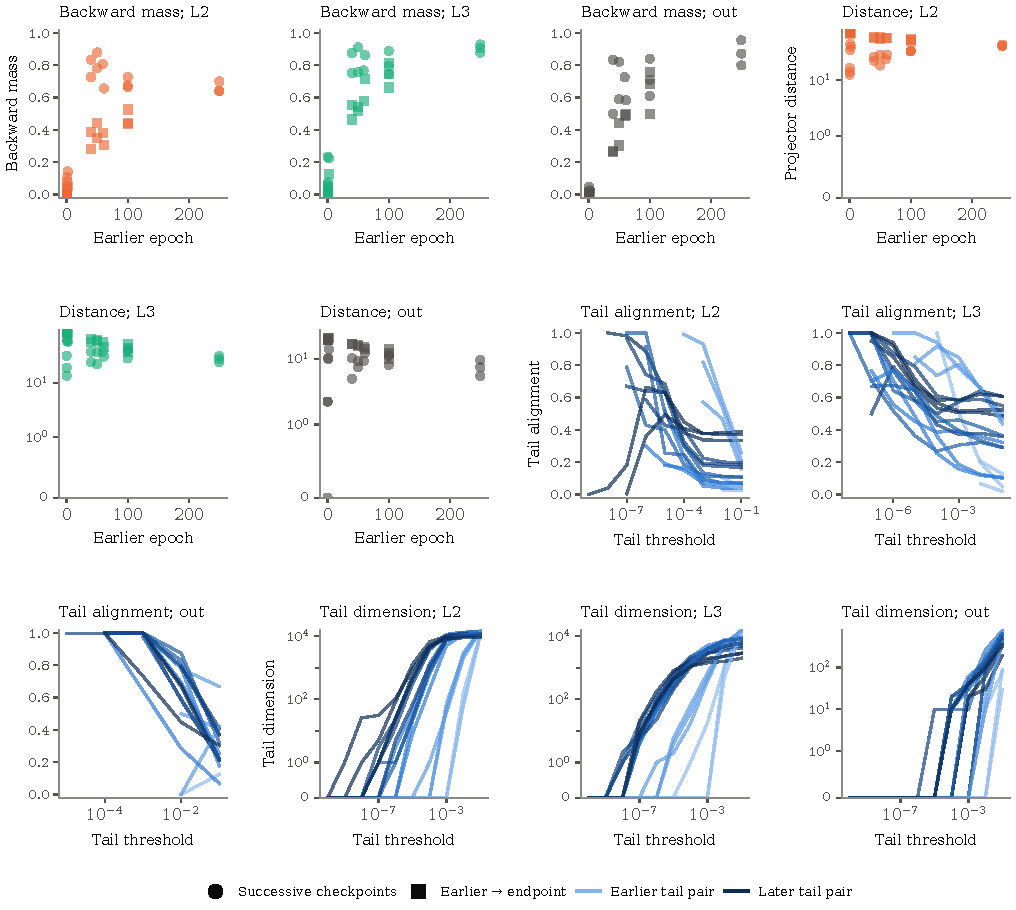
\includegraphics[width=6.096in]{persistence_tails.pdf}
\caption{Growth and spectral-tail alignment in the width-128 ReLU MLP, all three seeds. Panels 1--3 show how much of the later kernel was already present earlier; panels 4--6 show the projector distance, for every recorded checkpoint pair. Panels 7--9 and 10--12 show the positive spectral tail, excluding the current numerical kernel: its mean squared projection into the next kernel and its dimension, over the complete threshold grid on $J/\sqrt{s}$. Each line is one seed and consecutive checkpoint pair; darker lines denote later pairs. Alignment is projected mass, not an exact intersection dimension.}\label{fig:persistence-tails}
\end{figure}
\FloatBarrier
